\begin{figure}[h!]
\centering
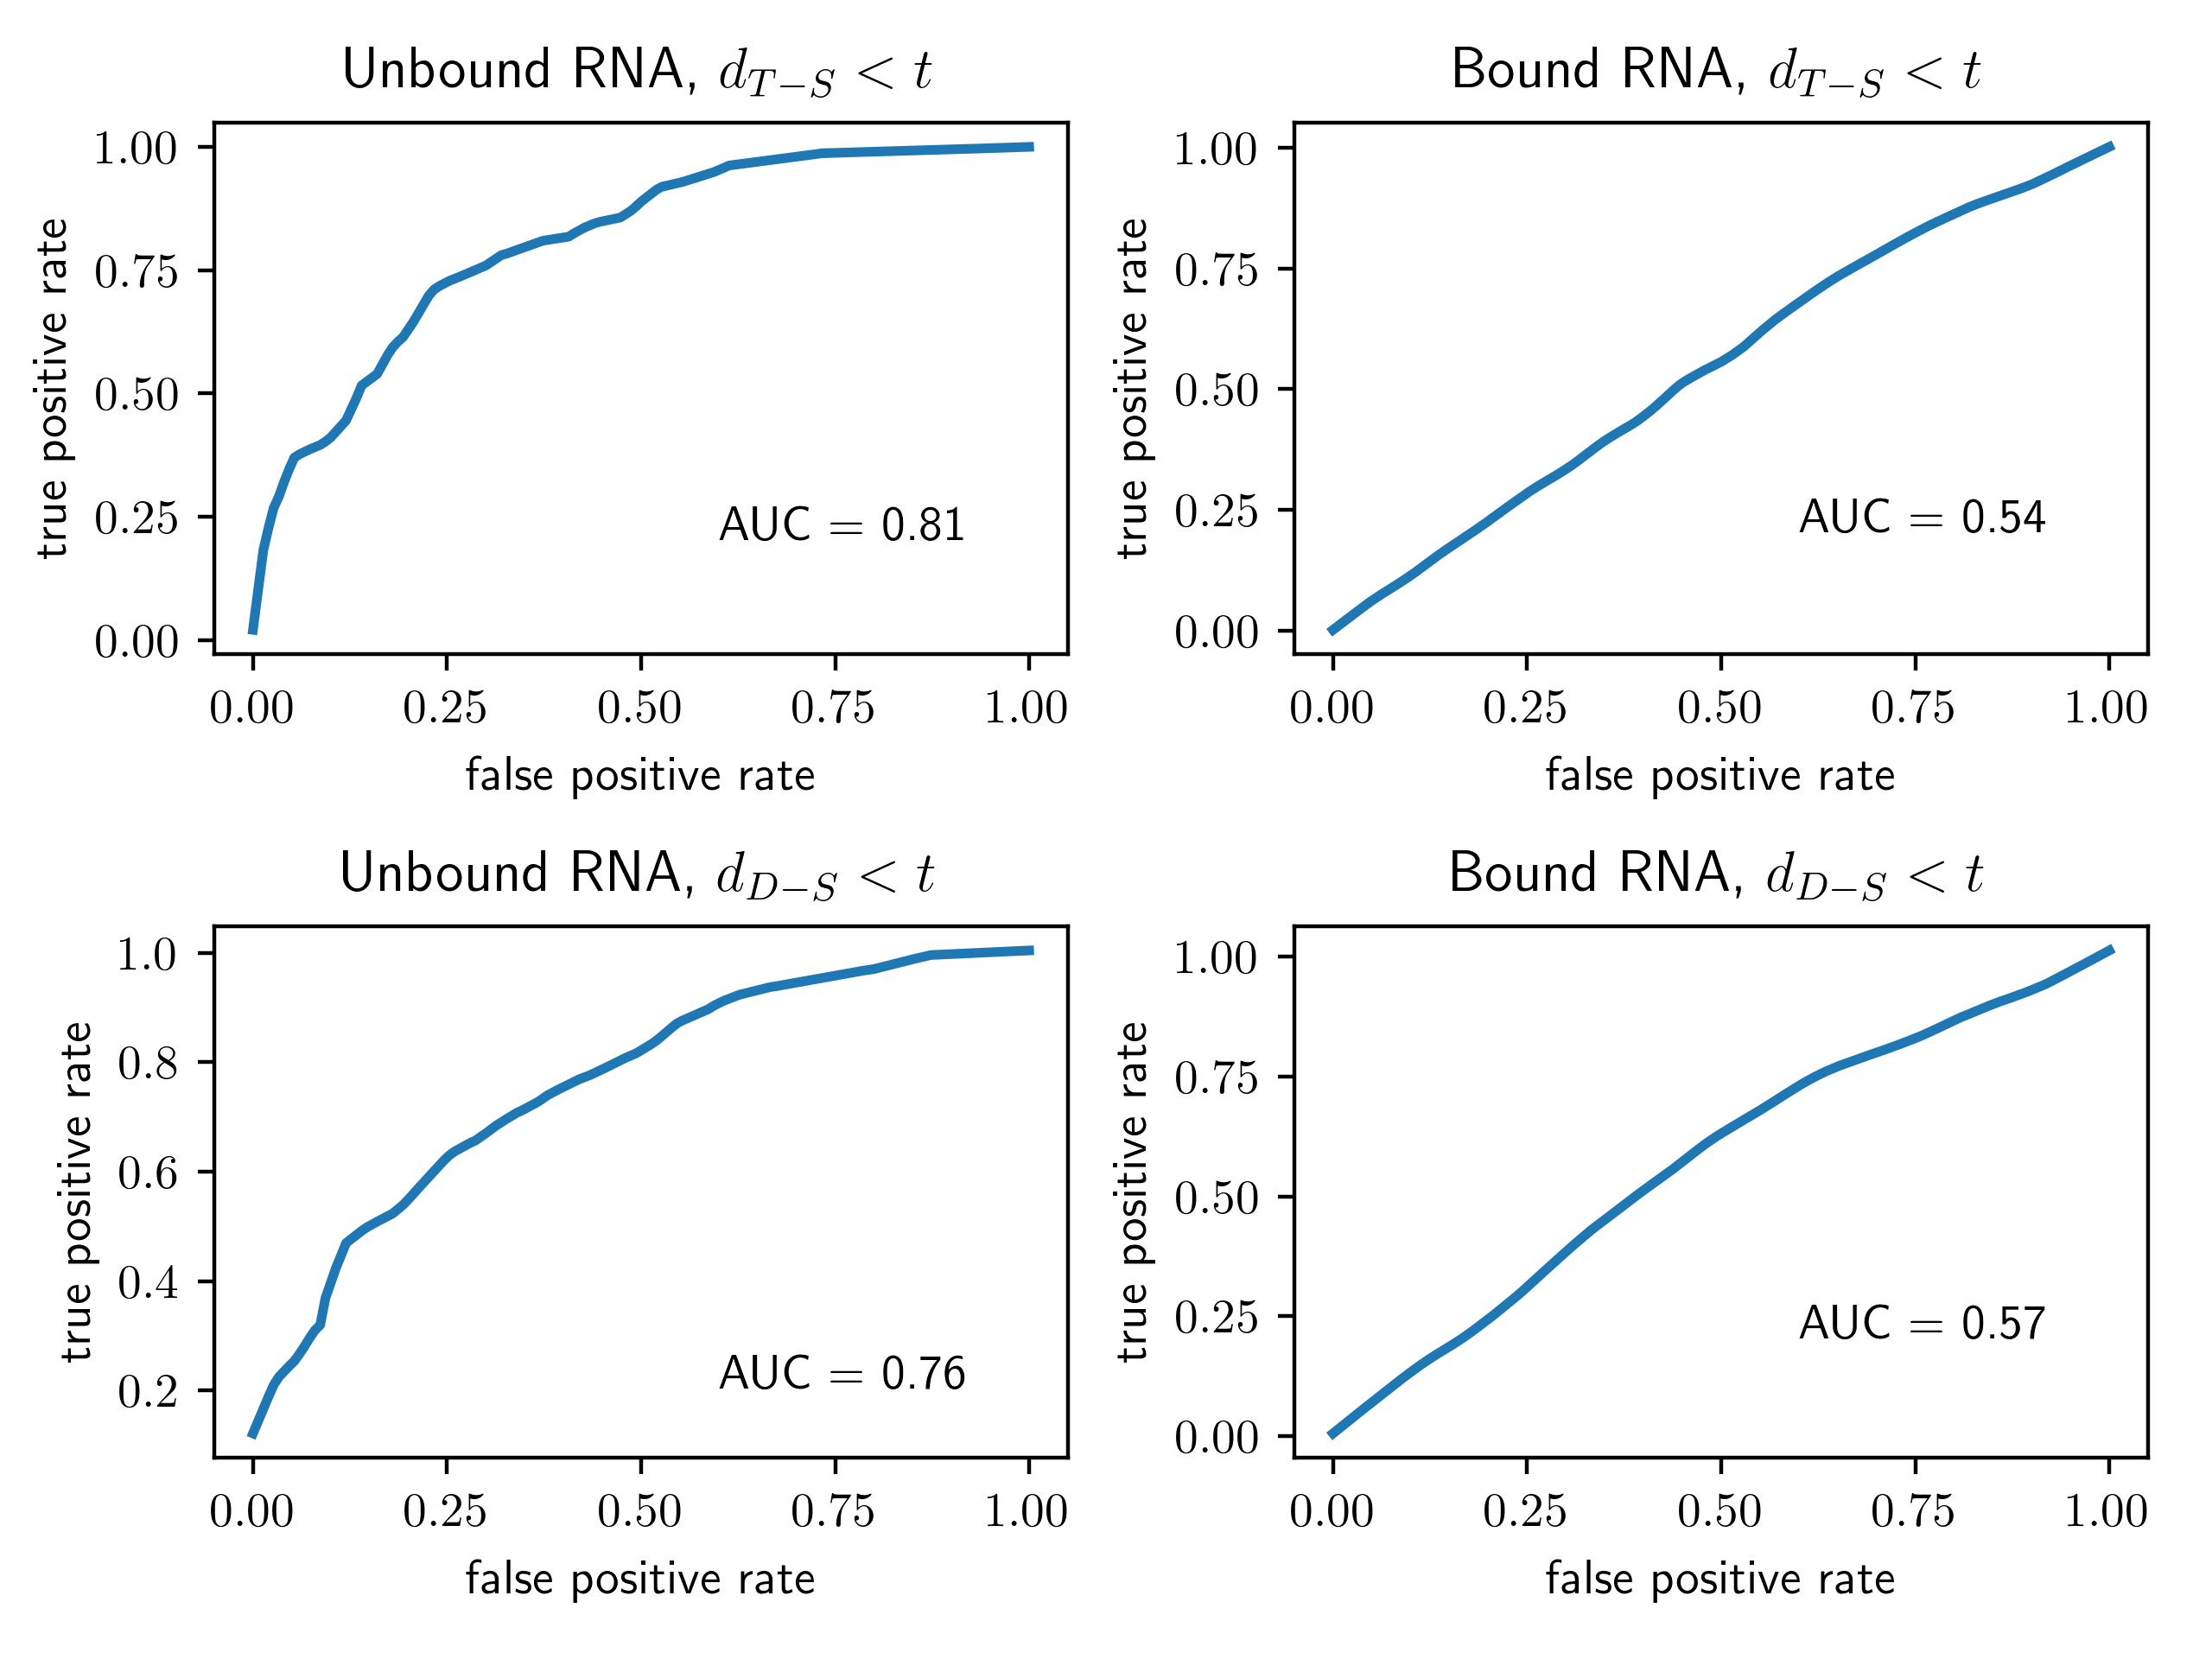
\includegraphics[width=\textwidth]{comparative_mfe.png}
\vglue 0.5cm

\caption{{\bf Comparative or MFE?} As in Figure \ref{fig:UnboundVSBound}, each panel
depicts the ROC performance of a classifier based on thresholding the T-S (top two panels) or
D-S (bottom two panels) ambiguity indexes. Here, small values are taken as evidence for
comparative as opposed to MFE secondary structure. Either index, T-S or D-S, can be used to
construct a good classifier of the origin of a secondary structure for the unbound molecules in
our data set (left two panels) but not for the bound molecules (right two panels). Conditional
p-values were also calculated, using the hypergeometric distribution and based only on the signs
of the indexes. In each case and the null hypothesis is that comparative secondary structures are as
likely to lead to positive ambiguity indexes as are MFE structures, whereas the alternative is
that positive ambiguity indexes are more typical when derived from MFE structures:
{\em Upper Left:} $p= 5.4 \times 10^{-14} $; {\em Upper Right:} $p=0.07$; {\em Lower Left:} $p=3.8 \times 10^{-7}$;  {\em Lower Right:} $p=0.01$.}
\label{fig:CompVSMFE}
\end{figure}
